\iffalse
    \title{2020}
    \author{EE24BTECH11001}
    \section{mcq-single}
\fi
	\item
		Let two points be A$\brak{1, -1}$ and B$\brak{0, 2}$. If a point P$\brak{x', y'}$ be
		such that area of $\Delta PAB = 5$sq. units and it lies if the line, $3x + y - 4\lambda = 0,$ then
		the value of $\lambda$ is :
		\hfill{\brak{2020-Jan}}
	\begin{multicols}{4}
		\begin{enumerate}
			\item 4 
			\columnbreak
			\item 1
			\columnbreak
			\item -3
			\columnbreak
			\item 3
		\end{enumerate}
	\end{multicols}

	\item The shortest distance between the lines
		\begin{align*}
		\frac{x-3}{3} = \frac{y-8}{-1} = \frac{z-3}{-1}
		\end{align*} And
		\begin{align}
			\frac{x+3}{3} = \frac{y+7}{2} = \frac{z-6}{1}
		\end{align}
		\hfill{\brak{2020-Jan}}
	\begin{multicols}{4}
		\begin{enumerate}
			\item $2\sqrt{30}$ \columnbreak
			\item $\frac{7\sqrt{30}}{2}$ \columnbreak
			\item 3 \columnbreak
			\item $3\sqrt{30}$
		\end{enumerate}
	\end{multicols}


\item Let the line $y = mx$ and the ellipse $2x^2 + y^2 = 1$ intersect a point $P$ in the first quadrant. If the 
	normal to this ellipse at $P$ meets the co-ordinate axes at $\brak{\frac{-1}{3\sqrt{2}}, 0}$ and $\brak{0, \beta}$
	, then $\beta$ is equal to 
		\hfill{\brak{2020-Jan}}
		\begin{enumerate}
			\begin{multicols}{2}
			\item $\frac{2}{\sqrt{3}}$ \columnbreak
			\item $\frac{2}{3}$
			\end{multicols}
			\begin{multicols}{2}
			\item $\frac{2\sqrt{2}}{3}$ \columnbreak
			\item $\frac{\sqrt{2}}{3}$
			\end{multicols}
		\end{enumerate}
		\begin{figure}
			\centering
		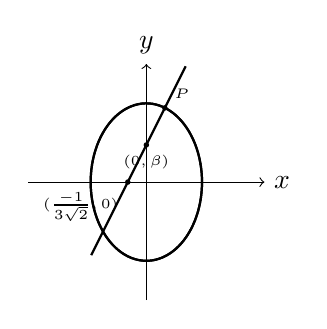
\begin{tikzpicture}
    			\draw[black, thick, domain=0:360, samples=100] 
        			plot ({sqrt(1/2)*cos(\x)}, {sin(\x)}); 
    			\draw[black, thick, domain=0:360, samples=100] 
        			plot ({sqrt(1/2)*cos(\x)}, {-sin(\x)}); 
    
    			\draw[->] (-1.5, 0) -- (1.5, 0) node[right] {$x$};
    			\draw[->] (0, -1.5) -- (0, 1.5) node[above] {$y$};
    
    
    			\draw[black, thick, domain=-0.7:0.5, samples=100]
        			plot ({\x}, {2*(\x) + 0.4714});
    
    			\fill[black] (0, 0.4714) circle (1pt) node[below] {\tiny $(0, \beta)$};
    			\fill[black] ({-1/(3*sqrt(2))}, 0) circle (1pt) node[below left] {\tiny $(\frac{-1}{3\sqrt{2}}, 0)$};
    			\fill[black] (0.235, 0.942) circle (1pt) node[above right] {\tiny $P$};		
		\end{tikzpicture}
		\end{figure}
	\item If $c$ is a point at which Rolle's Theorem holds for the function,
		\begin{align}
			f(x) = \log_e \brak{\frac{x^2 + \alpha}{7x}}
		\end{align}
		in the interval $\brak{3, 4}$, where $\alpha \in R$, then $f''(c)$ is equal to : 

		\hfill{\brak{2020-Jan}}
		\begin{enumerate}
			\begin{multicols}{4}
				\item $\frac{-1}{24}$ \columnbreak
				\item $\frac{-1}{12}$ \columnbreak
				\item $\frac{\sqrt{3}}{7}$ \columnbreak
				\item $\frac{1}{12}$
			\end{multicols}
		\end{enumerate}

	\item Let
		\begin{align}
			f\brak{x} = x \cos ^{-1}\brak{\sin \brak{-|x|}}, x \in \brak{\frac{-\pi}{2}, \frac{\pi}{2}}
		\end{align}, then which of the following is true
		
		\hfill{\brak{2020-Jan}}
		\begin{enumerate}
			\item $f\brak{0} = \frac{-\pi}{2}$ 
			\item $f'$ is decreasing in $\brak{\frac{-\pi}{2}, 0}$ and increasing in $\brak{0, \frac{\pi}{2}}$ 
			\item $f$ is not differentiable at $x = 0$  
			\item $f'$ is increasing in $\brak{\frac{-\pi}{2}, 0}$ and decreasing in $\brak{0, \frac{\pi}{2}}$
		\end{enumerate}


